\documentclass[a4paper,12pt]{article}

\usepackage[top=3cm, bottom=2cm, left=3cm, right=2cm]{geometry}
\usepackage[utf8]{inputenc}
\usepackage[portuguese]{babel}
\usepackage{booktabs}
\usepackage{multirow}
\usepackage{hyperref}
\usepackage{graphicx}
\usepackage{longtable}
\usepackage{verbatim}
\usepackage{url}
\usepackage{morefloats}

\usepackage{float}
\floatstyle{ruled}
\newfloat{program}{thp}{lop}
\floatname{program}{Log}
\newfloat{config}{thp}{lop}
\floatname{config}{Configuração}

\title{Serviços de Rede e de Sistema \\
Desenhar e correr um serviço de E-mail}

\author{André Fernandes (ei03107) \and Miguel Gomes (ei07075) \and Pedro Batista (ext10392)}

\begin{document}

\maketitle

\section{Topologia}

Em virtude da configuração DNS do laboratório estar {\bf incorrecta} decidimos 
mudar a topologia da rede conforme a figura \ref{fig:topologia}.
Esta alteração deveu-se ao facto de nem a máquina denominada por carvoeiro no 
guião (192.168.109.2), nem as máquinas com os IP 193.136.28.10 e 172.16.2.2 
presentes na rede, constarem de serviços DNS que conhecessem, simultaneamente,
os registo MX e A dos GNUs.

Mais especificamente, os serviços DNS do carvoeiro e da máquina 172.16.2.2 
conheciam o registo MX, mas não conhecia o endereço dos GNUs. Já o 
serviço DNS da máquina 193.136.28.10 conhecia os endereços dos GNUs mas 
não conhecia os registos MX.

Estas afirmações podem ser confirmadas pelos logs \ref{log:carvoeiromx}, 
\ref{log:carvoeiroa}, \ref{log:193a}, \ref{log:193mx}, \ref{log:172mx}
e \ref{log:172a}.

Embora a topologia implementada ter sido diferente do guião achámos que a
topologia não foi alterada signitivamente face ao objectivo trabalho proposto.

O trabalho realizado diferiu, essencialmente, em dois aspectos. Em primeiro
lugar, com o facto dos computadores estarem ligados directamente ao mesmo
switch. E em segundo, pelo domínio \emph{psb.com} ter sido configurado
numa máquina que chamámos de ``pa'' e que serviu como cliente
pop3 e imap.

\begin{figure}[htp]
	\begin{center}
		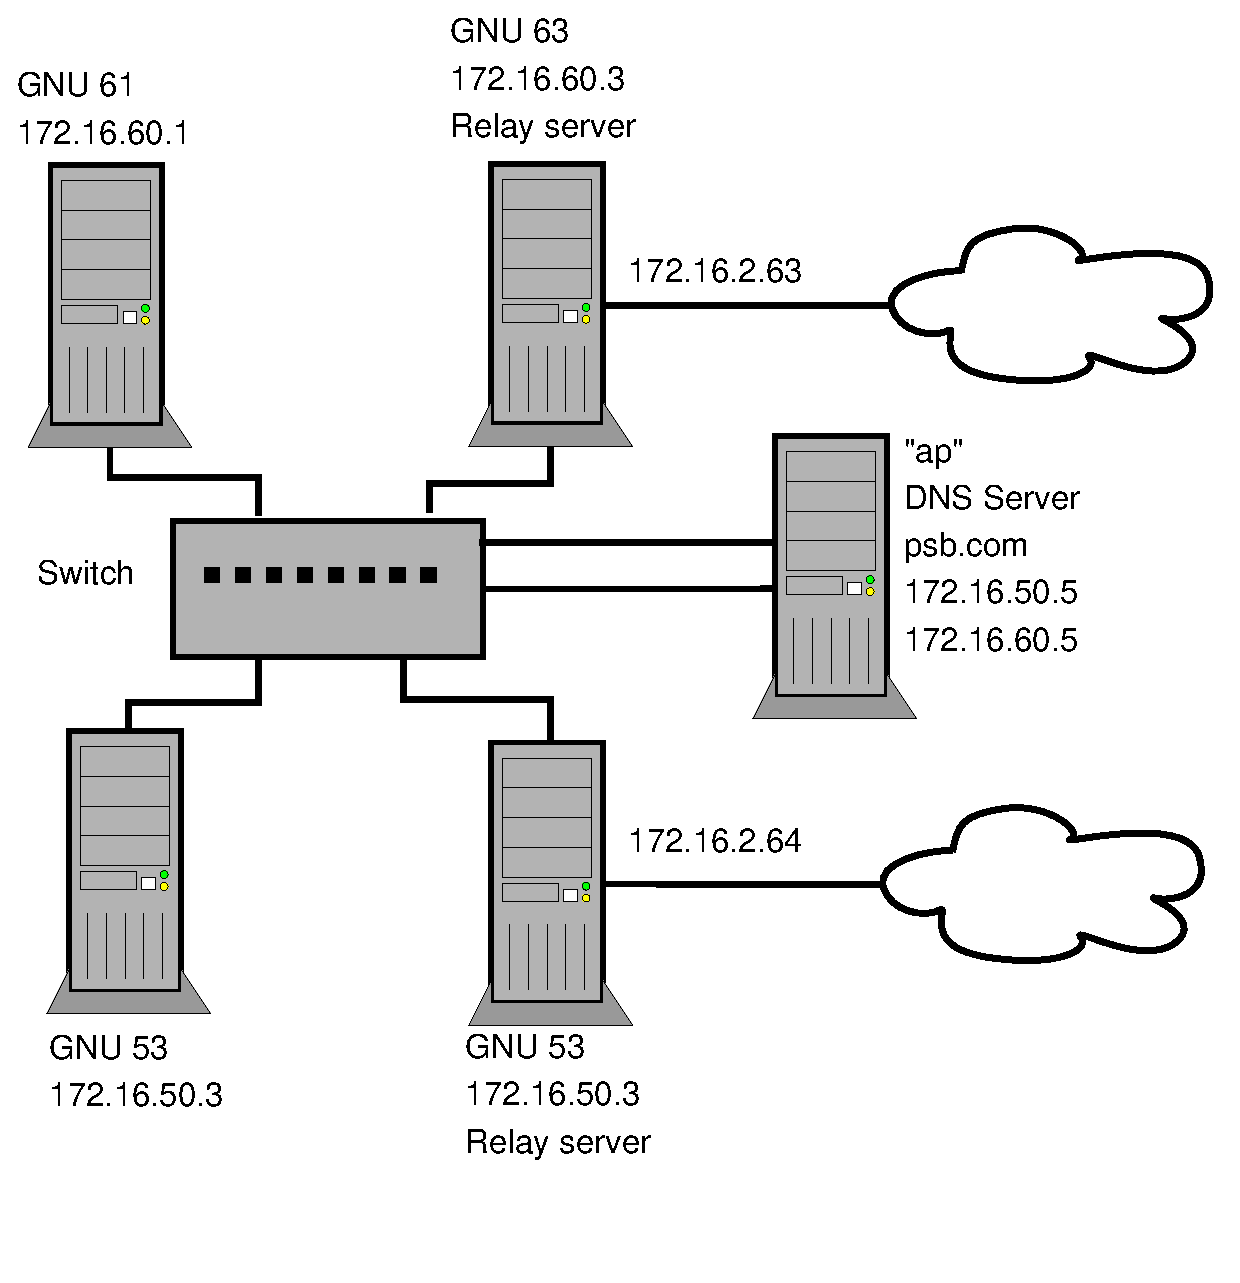
\includegraphics[height=6in]{topologia}
	\end{center}
	\caption{Topologia de rede implementada.}
	\label{fig:topologia}
\end{figure}

\begin{program}
	\verbatiminput{carvoeiro_mx}
  \caption{Pergunta ao carvoeiro sobre o registo MX da bancada6.}
	\label{log:carvoeiromx}
\end{program}

\begin{program}
	\verbatiminput{carvoeiro_a}
  \caption{Pergunta ao carvoeiro sobre o registo do GNU63.}
	\label{log:carvoeiroa}
\end{program}

\begin{program}
	\verbatiminput{193_mx}
  \caption{Pergunta à máquina 193.136.28.10 sobre o registo MX da bancada6.}
	\label{log:193mx}
\end{program}

\begin{program}
	\verbatiminput{193_a}
  \caption{Pergunta à máquina 193.136.28.10 sobre o registo do GNU63.}
	\label{log:193a}
\end{program}

\begin{program}
	\verbatiminput{172_mx}
  \caption{Pergunta à máquina 172.16.2.2 sobre o registo MX da bancada6.}
	\label{log:172mx}
\end{program}

\begin{program}
	\verbatiminput{172_a}
  \caption{Pergunta à máquina 172.16.2.2 sobre o registo do GNU63.}
	\label{log:172a}
\end{program}


\section{Configurações}

Os ficheiros das configurações encontram-se em anexo no arquivo ``conf''.
Dentro deste arquivo encontram-se pastas com o nome ``gXY'' com os ficheiros
de configuração para cada ``GNUXY''. Adicionalmente, encontra-se ainda um
arquivo com o nome ``pa'' com as configurações do servidor DNS presente na 
figura \ref{fig:topologia}.

\section{Registo de Logs}

Com o objectivo de registar o tráfego completo da rede configurámos uma porta
do switch como uma porta SPAN (Switched Port Analyzer) por forma a escutar todo
o tráfego da rede no Wireshark.
Uma vez que os arquivos das capturas são de grande dimensão decidímos anexar 
ao relatório um arquivo com todos estes registos com o nome de ``wireshark''. 
A sessões encontram-se organizadas como se segue:

\begin{itemize}
	\item Sessão 1 - Tráfego de SMTP dentro da bancada 6.
	\item Sessão 2 - Tráfego de SMTP da bancada 6 para a bancada 5.
	\item Sessão 3.1 - Tráfego POP3.
	\item Sessão 3.2 - Tráfego POP3 SSL.
	\item Sessão 4.1 - Tráfego IMAP.
	\item Sessão 4.2 - Tráfego IMAP SSL.
	\item Sessão 5.1 - Mail do user1 da bancada 6 para o user2 da bancada 6.
	\item Sessão 5.2 - Mail do user2 da bancada 6 para o netedu da bancada 6.
	\item Sessão 5.3 - Mail do netedu da bancada 6 para o user1 da bancada 6.
	\item Sessão 5.4 - Mail do user1 da bancada 5 para o user1 da bancada 6.
	\item Sessão 5.5 - Mail do user1 da bancada 5 para o user2 da bancada 6.
	\item Sessão 5.6 - Mail do user1 da bancada 5 para o netedu da bancada 6.
\end{itemize}

\section{Análise de resultados}


\section{Conclusão}

Neste trabalho foi possível comprovar a utilização do protocolo SMTP no 
envio de e-mails para o serviço Postfix. E, quase em simultâneo, verificar 
a utilização dos protocolos POP3 e IMAP no download de e-mails do 
serviço Postfix.
Também observámos a forma como os diversos serviços de SMTP colaboram na
troca de mensagens por forma às mesmas chegarem ao destino apropriado.
Adicionalmente, podemos observar através das capturas do Wireshark, que
quando o protocolo POP3 ou IMAP são utilizados sobre SSL, todas as
mensagens trocadas com o serviço Postfix são encriptadas. O que provoca
um overhead na comunicação entre Postfix e cliente de e-mail.

\end{document}
